\providecommand{\graphTheoryPreambleLoaded}{}
\ifx\graphTheoryPreambleLoaded
\documentclass{article}
\usepackage{./1_Preamble/graph_theory_preamble}

\begin{document}
	\fi
	
	\subsection*{Map Structure}
	\addcontentsline{toc}{subsection}{Map Structure}
	
	\subsubsection*{Game Map \& Chosen Area}
	\addcontentsline{toc}{subsubsection}{Game Map \& Chosen Area}
	Grand Theft Auto: San Andreas is by far, the second largest map area that one can explore at \(38.2\unit{\km}\)\footnote{https://www.sportskeeda.com/gta/gta-ranking-maps-order-size}. Only behind Grand Theft Auto V with an enormous total area of \(75.84\unit{\km}\)\footnote{Take the article with a grain of salt}.
	
	\begin{figure}[!h]
		\centering
		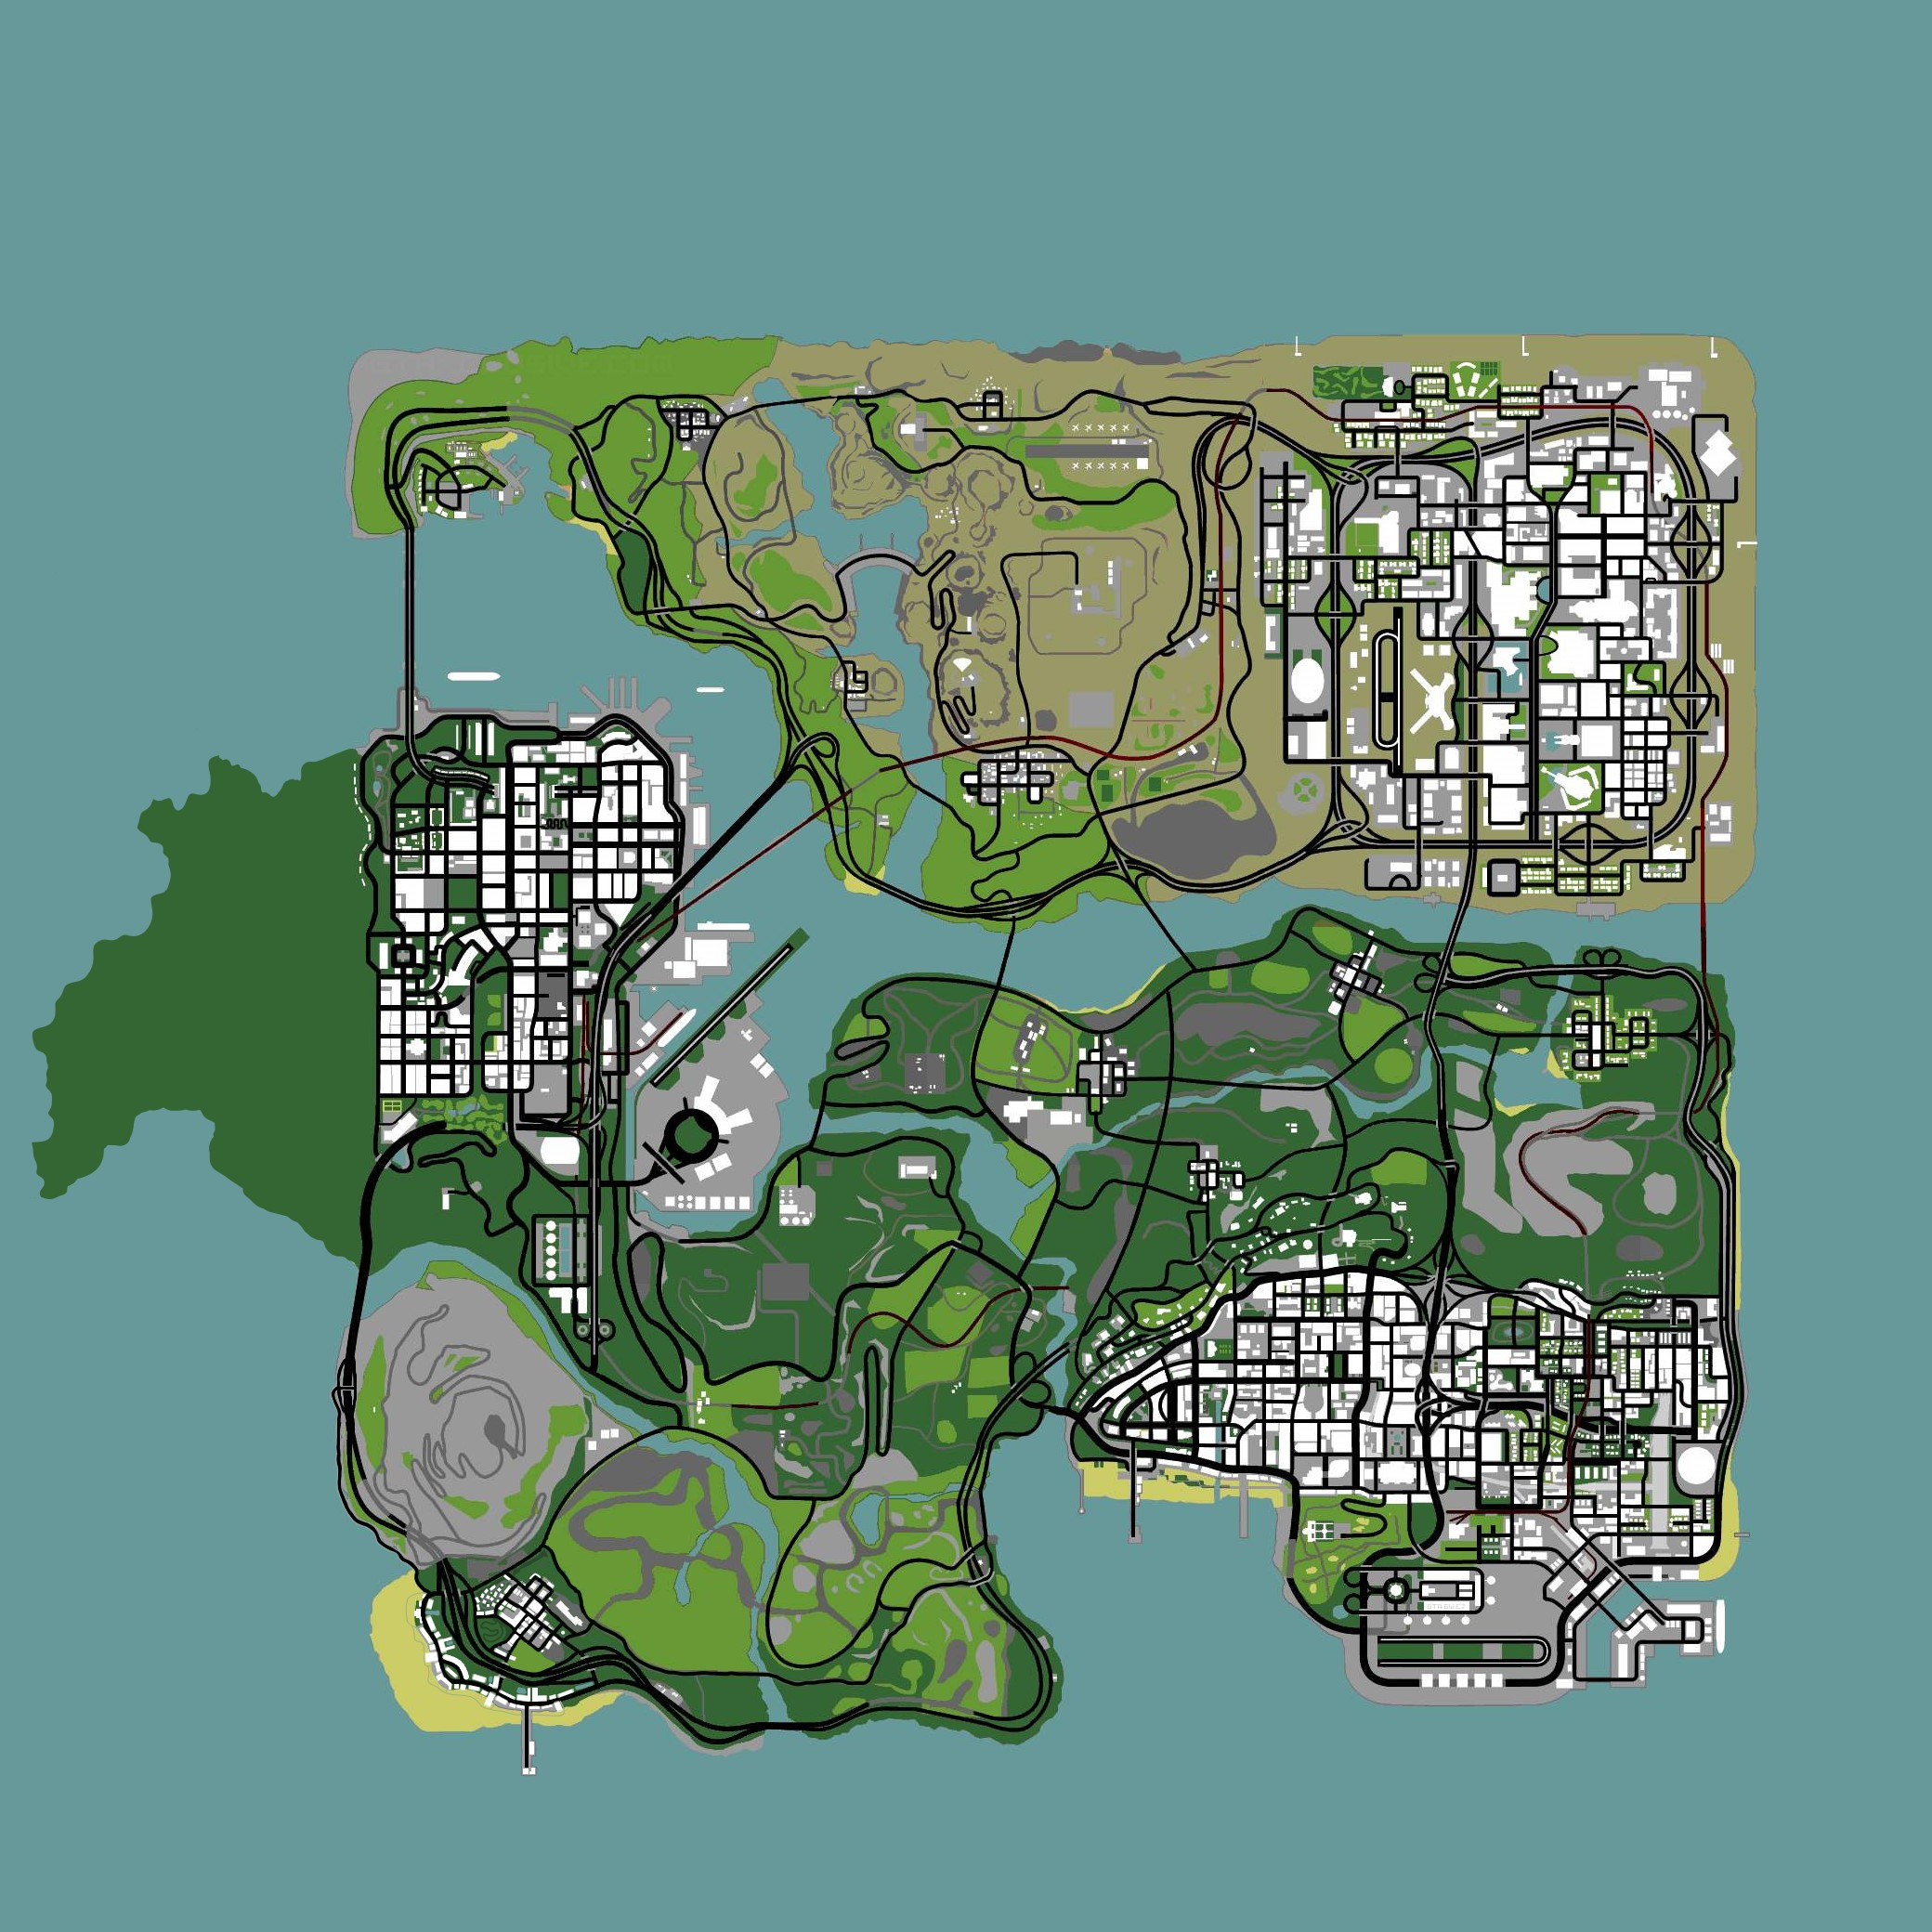
\includegraphics[width=0.75\textwidth]{./0img/gtaSAMap.jpg}
		\caption{Grand Theft Auto San Andreas Map \\ Taken From \href{https://gtaforums.com/topic/958639-gta-sa-map-improvements/}{\textcolor{green}{\underline{GTAForums}}}}
		\label{gtasa_map}
	\end{figure} This means we will instead focus on a specific region of the map. Particularly the area within Los Santos, can be found southeast in figure (\ref{gtasa_map}). We shall choose this region since it will be the first region to be unlocked when playing a new clean save [new game].
	
	\clearpage
	\begin{figure}[!h]
			\centering
			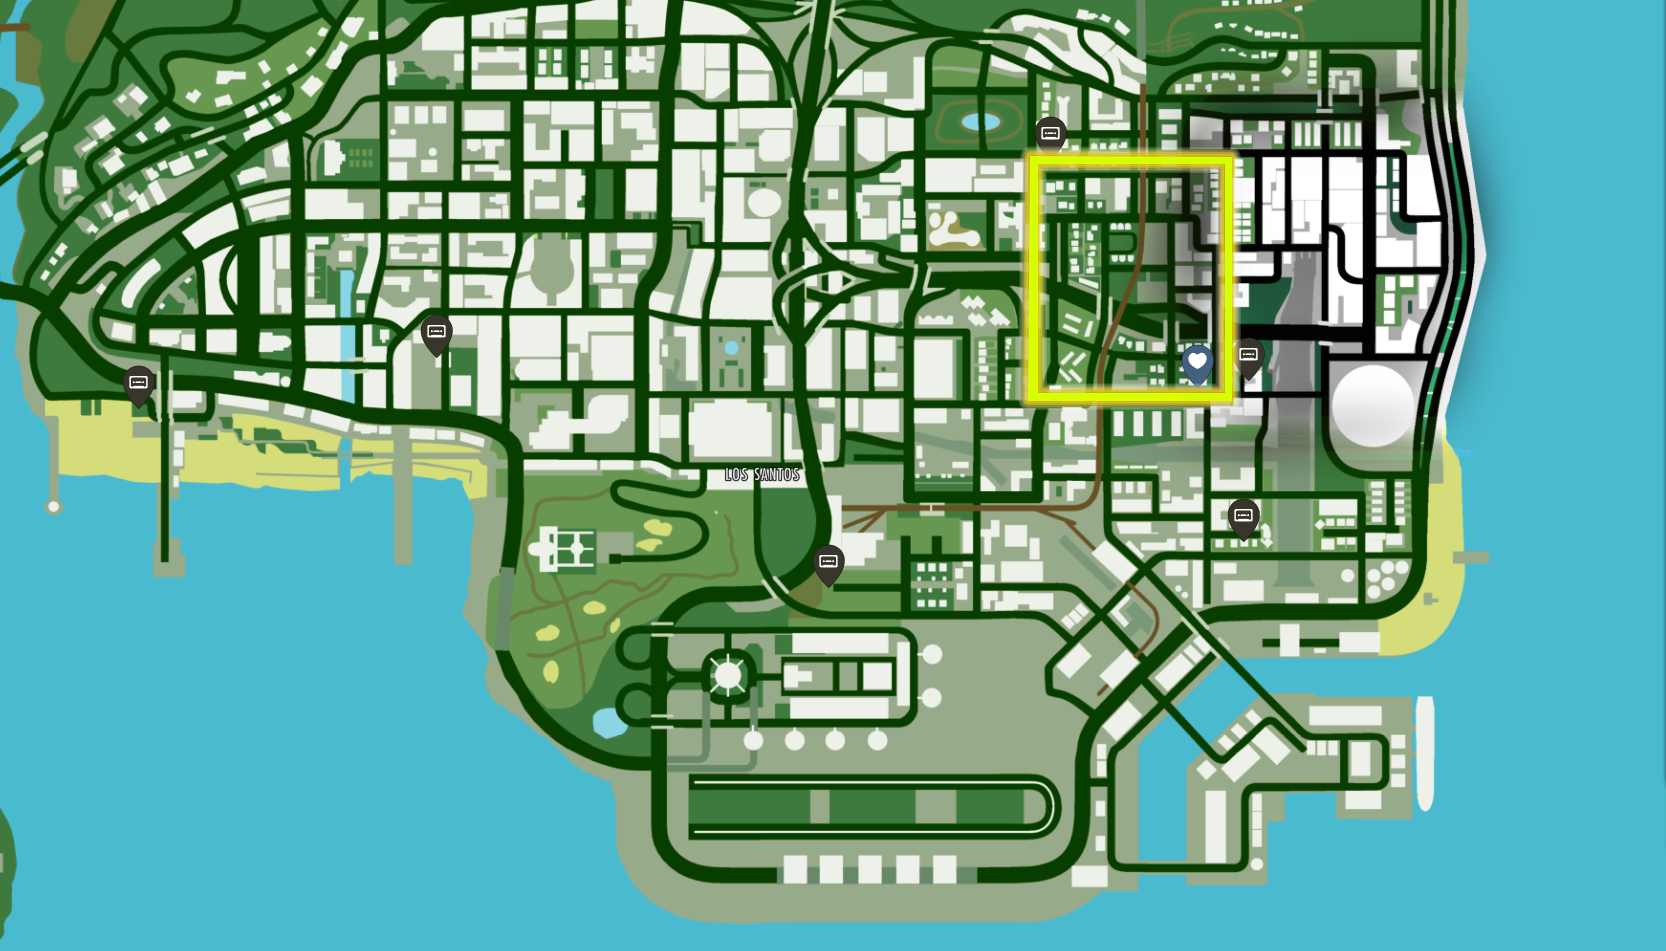
\includegraphics[width=0.85\textwidth]{./0img/gtaMap.png}
			\caption{Chosen Map Area in Los Santos \\ Highlighted in Yellow}
			\label{ls_map}
	\end{figure} Within the region of Los Santos we shall choose a specific area to create a graph analysis. In figure (\ref{ls_map}), when starting a new game, the player character will be situated on this area of the map. Most of the beginning missions will also be focused within its region. This means we shall choose due to having potential in exploration using graph theory. Instances may include:
	\begin{enumerate}
		\item Road Familiarity
		\item Collectible Hunting
		\item Spray Point Location
		\item Special Locations (Gym, Clothing Store, Safehouse, etc)
		\item Speedrunning Mission Locations
	\end{enumerate}
	
	\clearpage
	\subsubsection*{Location Placement}
	\addcontentsline{toc}{subsubsection}{Location Placement}
	There are heaps of combination as to how we will place the vertex of a map. What we will choose instead are the road corners or its meeting points.
	
	\begin{figure}[!h]
		\centering
		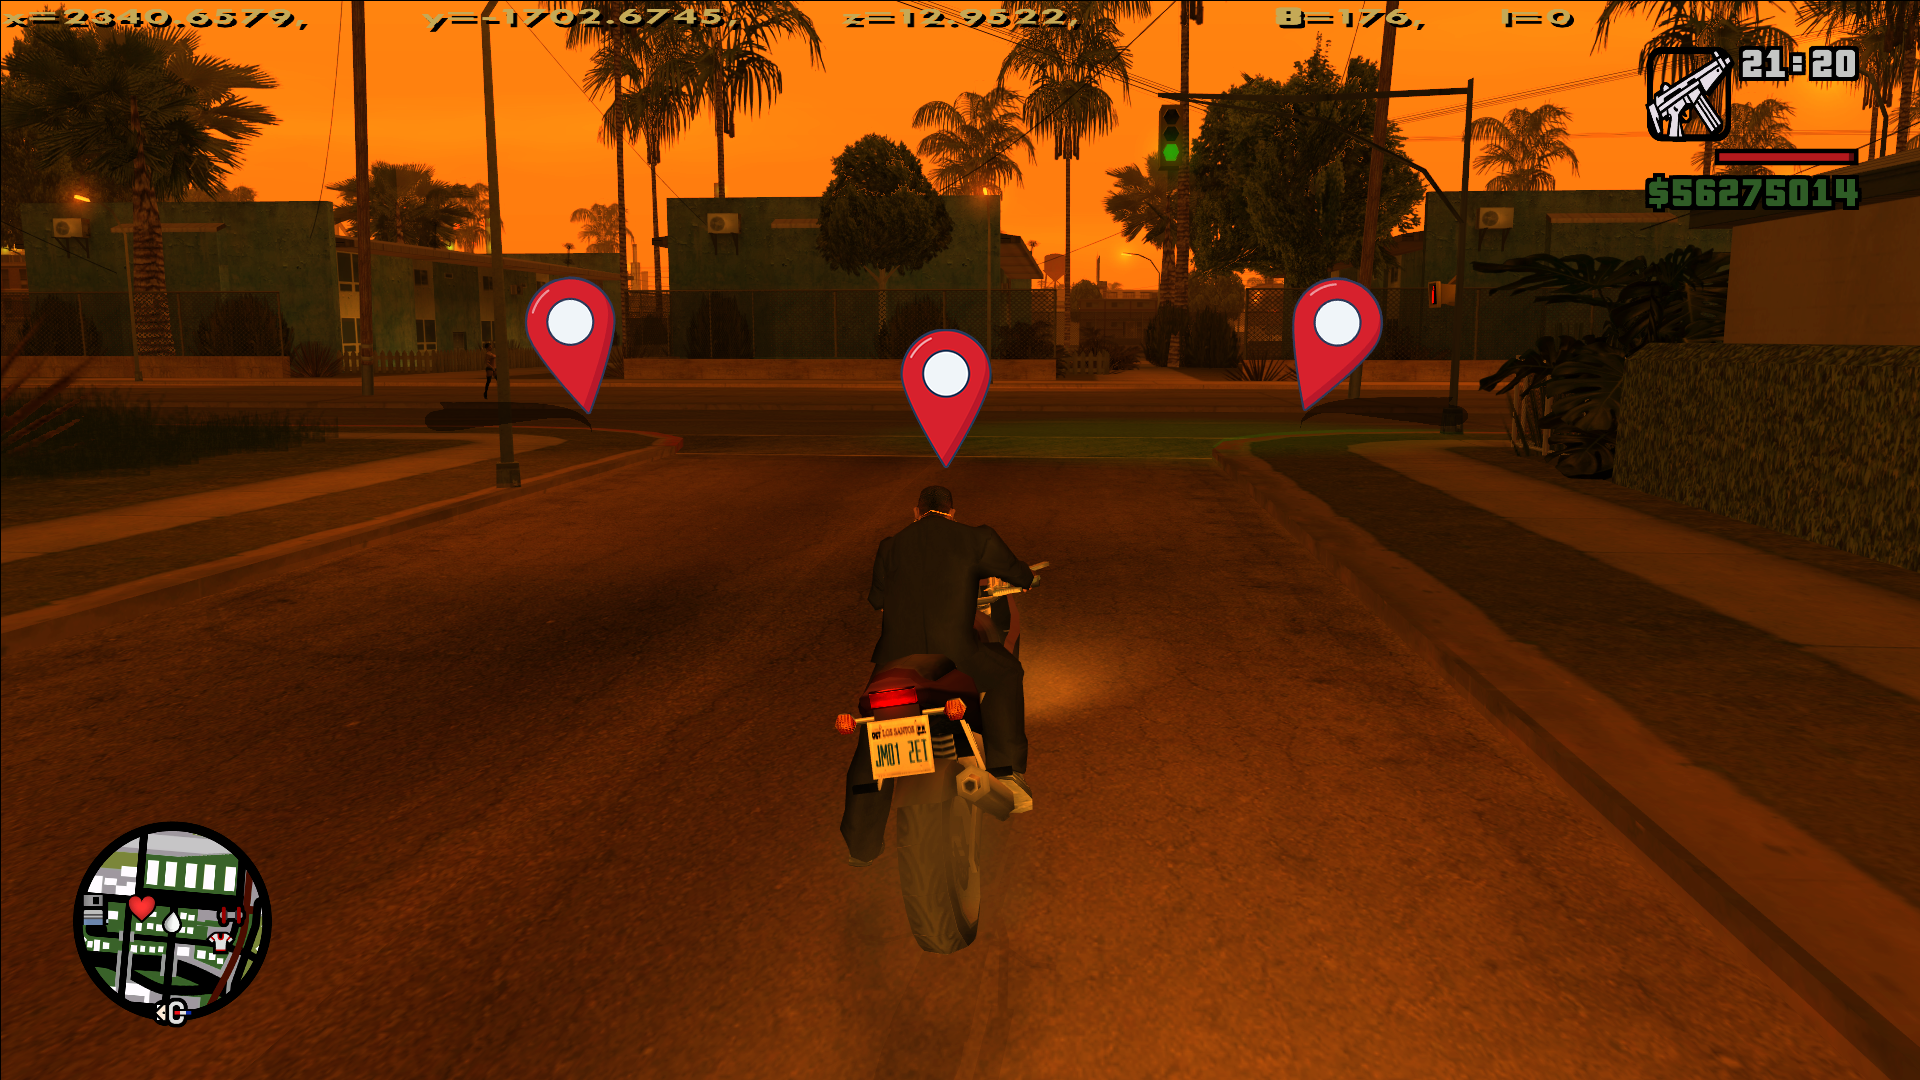
\includegraphics[width=1\textwidth]{./0img/locationPlacement.png}
		\caption{A T-intersection Location Placement}
	\end{figure} There is also two special locations that will be considered: One is the safehouse at Jefferson.
	
	\begin{figure}[!h]
		\centering
		\begin{minipage}{0.49\textwidth}
			\centering
			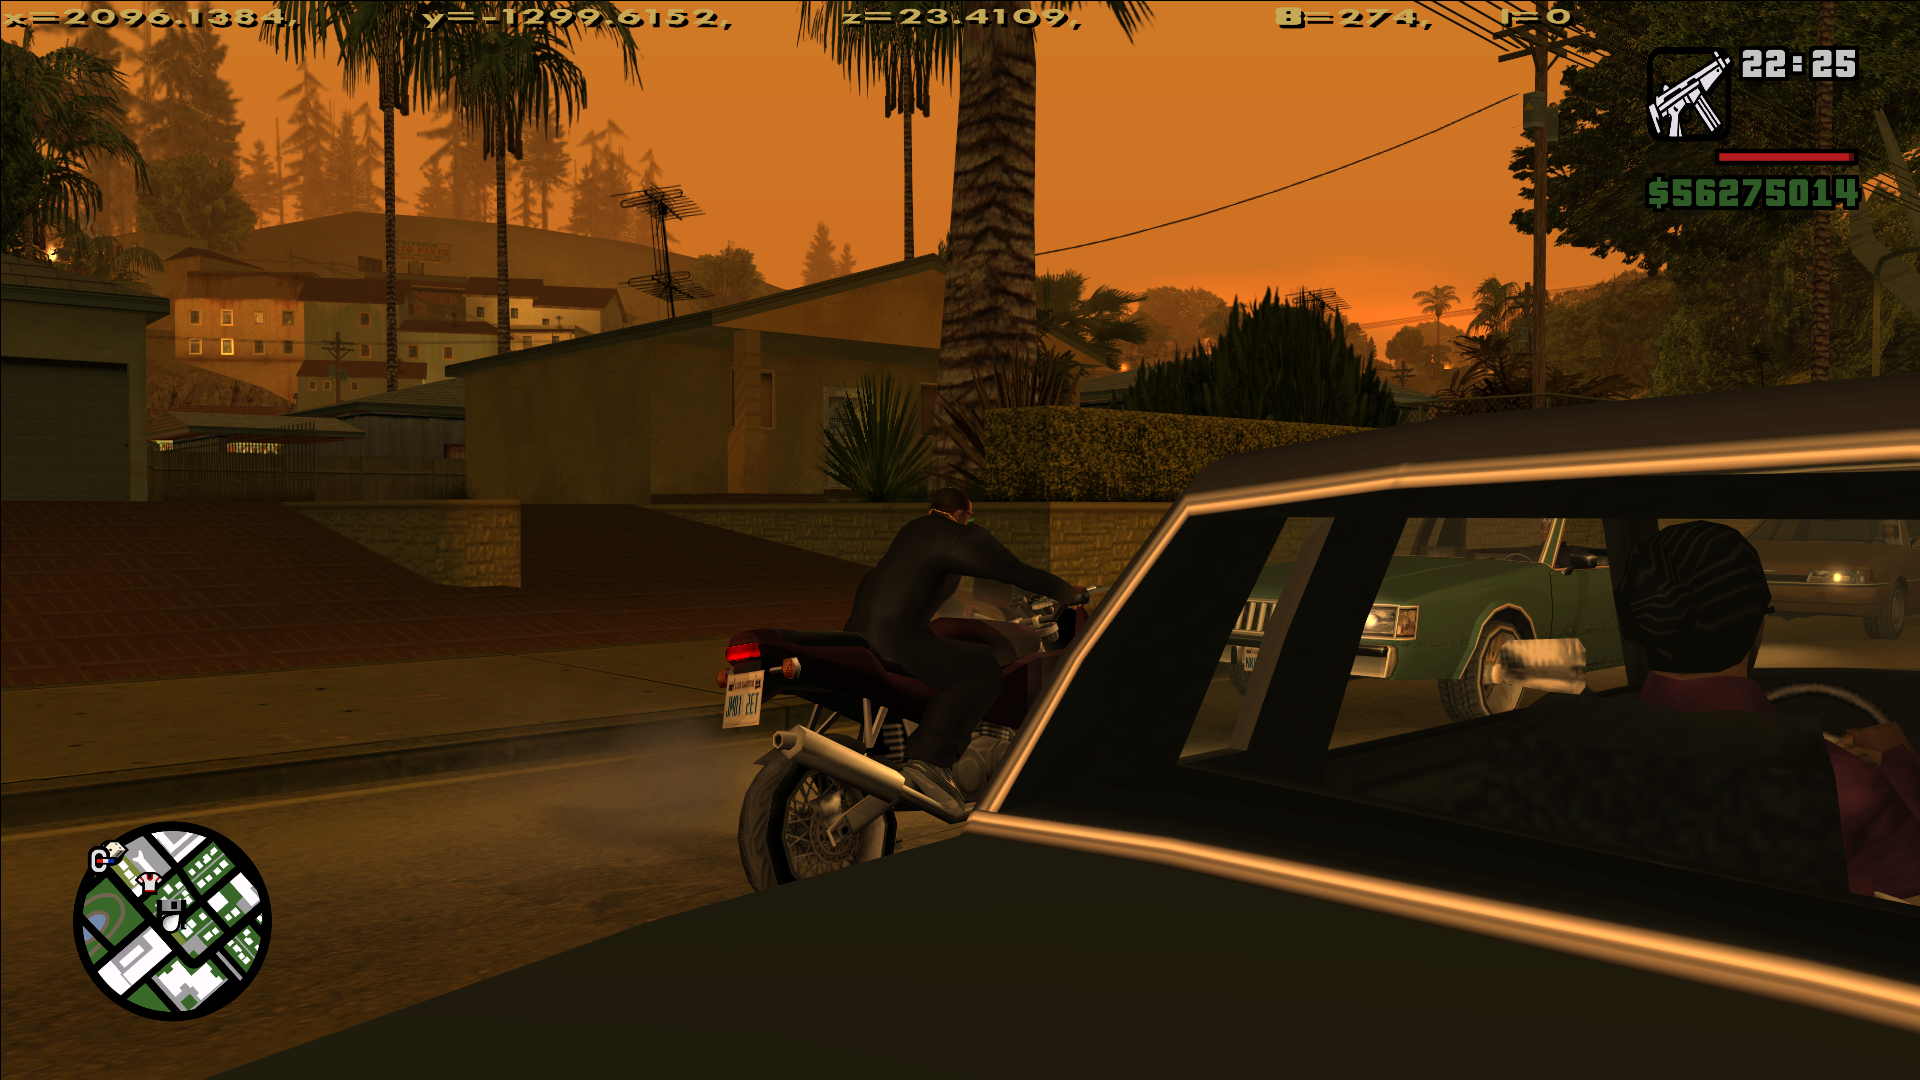
\includegraphics[width=1\textwidth]{./0img/safehouseLocation.png}
			\subcaption{Safehouse}
		\end{minipage}
		\hfill
		\begin{minipage}{0.49\textwidth}
			\centering
			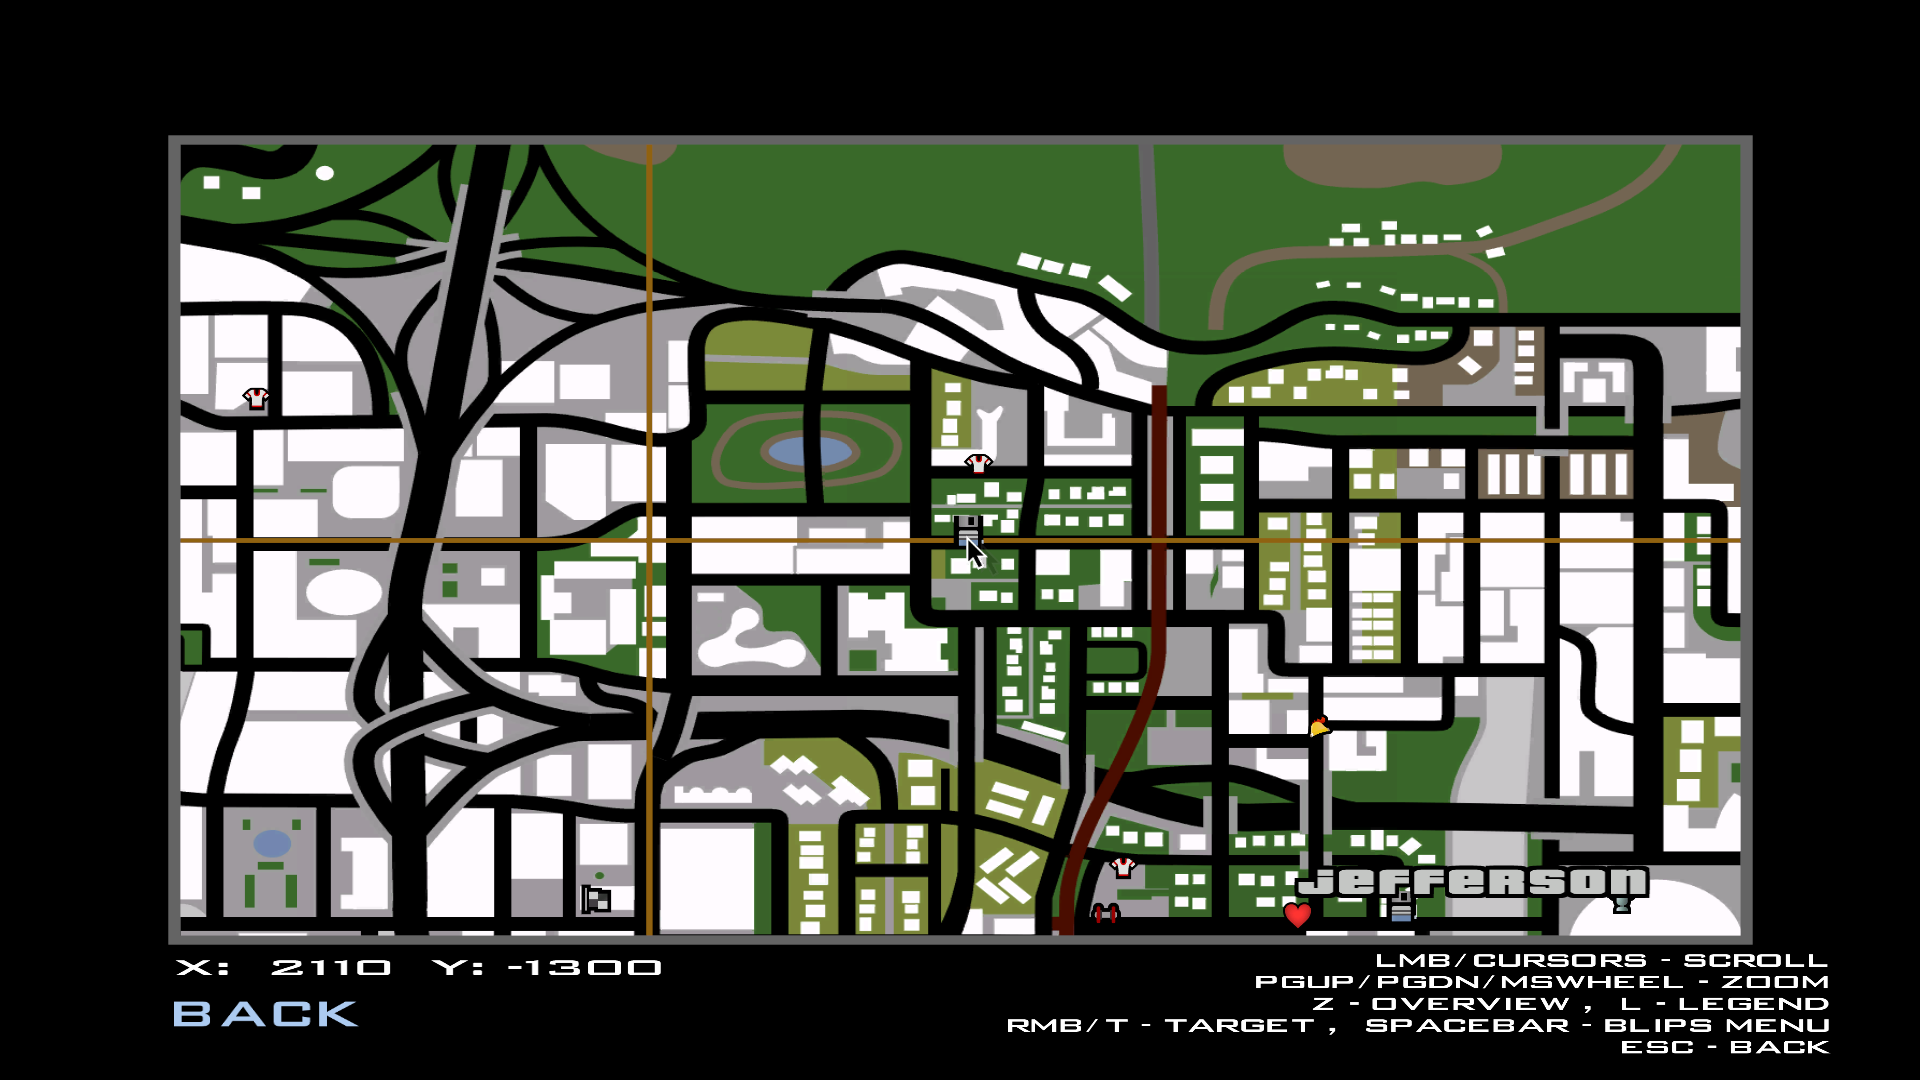
\includegraphics[width= 1\textwidth]{./0img/safehouseMap.png}
			\subcaption{Map Overview}
		\end{minipage}
		\caption{First Special Location}
	\end{figure} Then the player character's girlfriend's house at Ganton.
	
	\clearpage
	\begin{figure}[!h]
		\centering
		\begin{minipage}{0.49\textwidth}
			\centering
			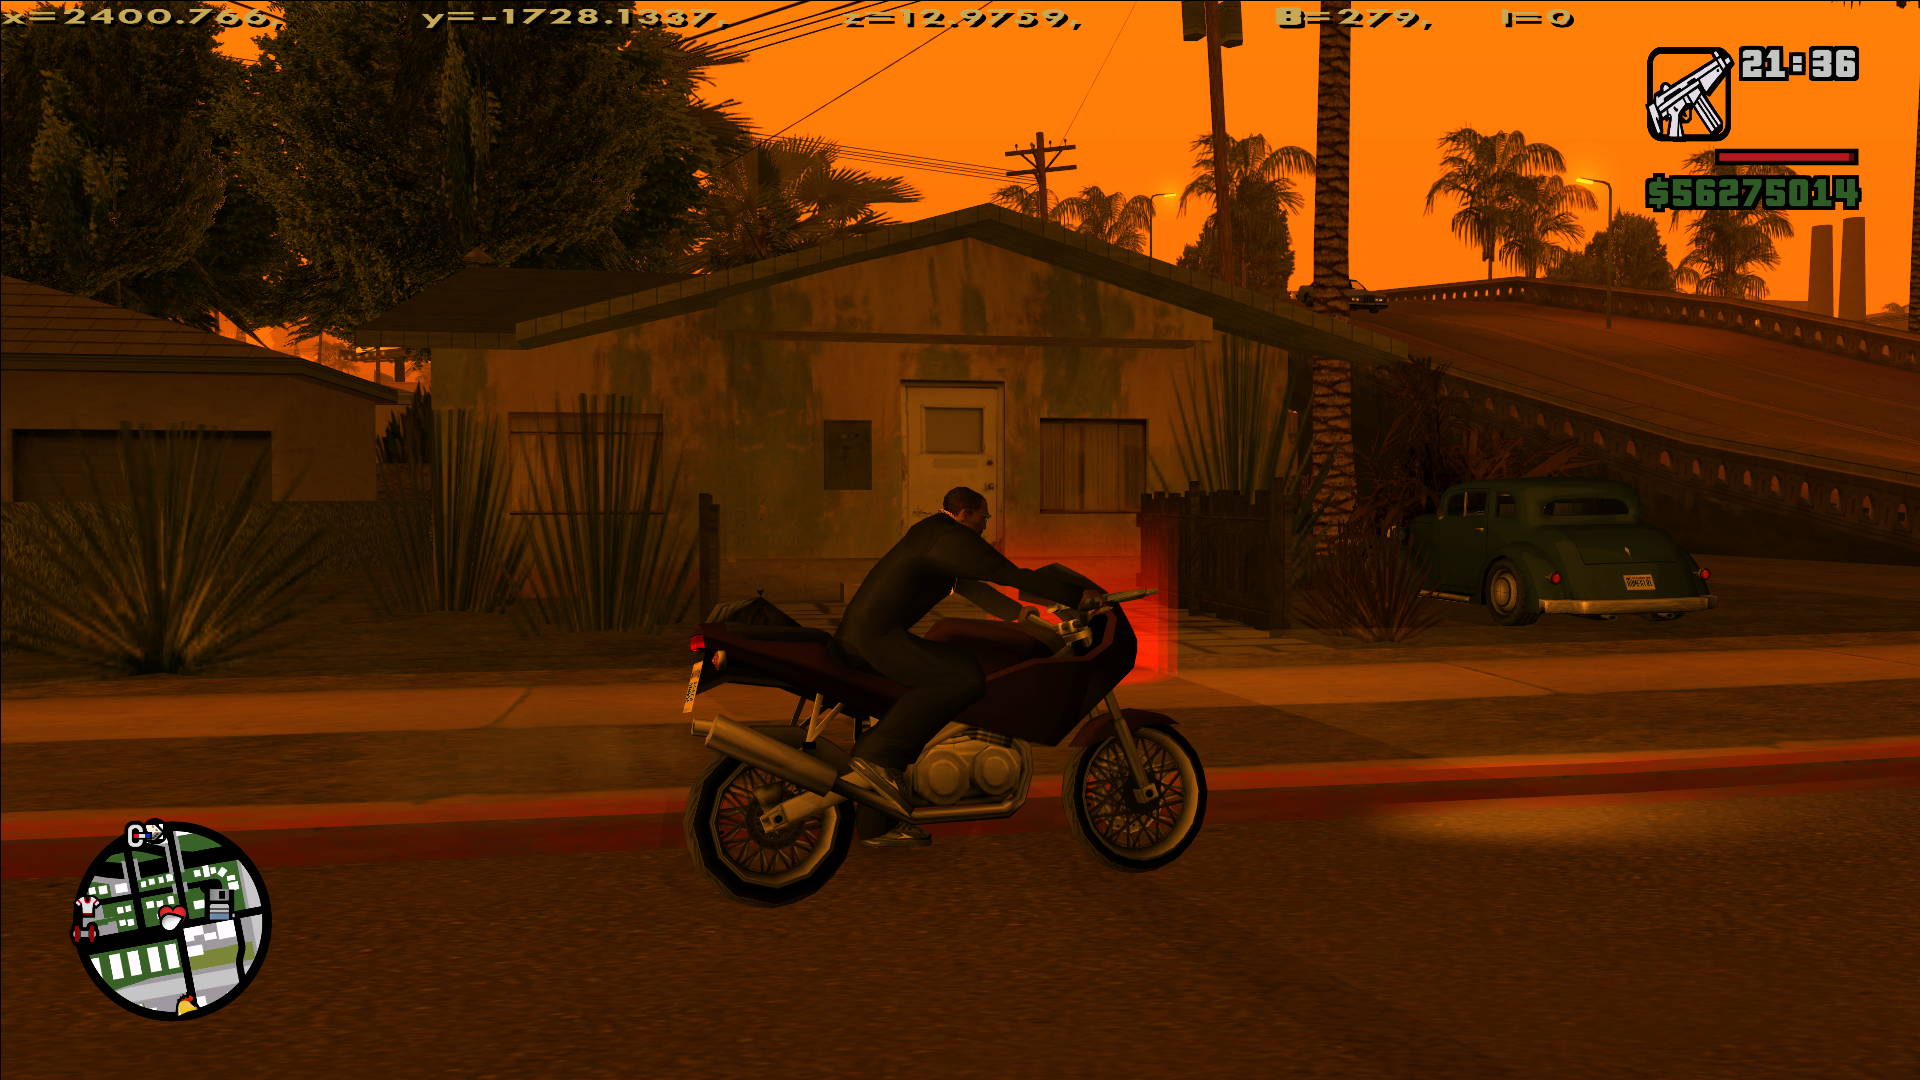
\includegraphics[width=1\textwidth]{./0img/girlfriendLocation.png}
			\subcaption{Girlfriend's House}
		\end{minipage}
		\hfill
		\begin{minipage}{0.49\textwidth}
			\centering
			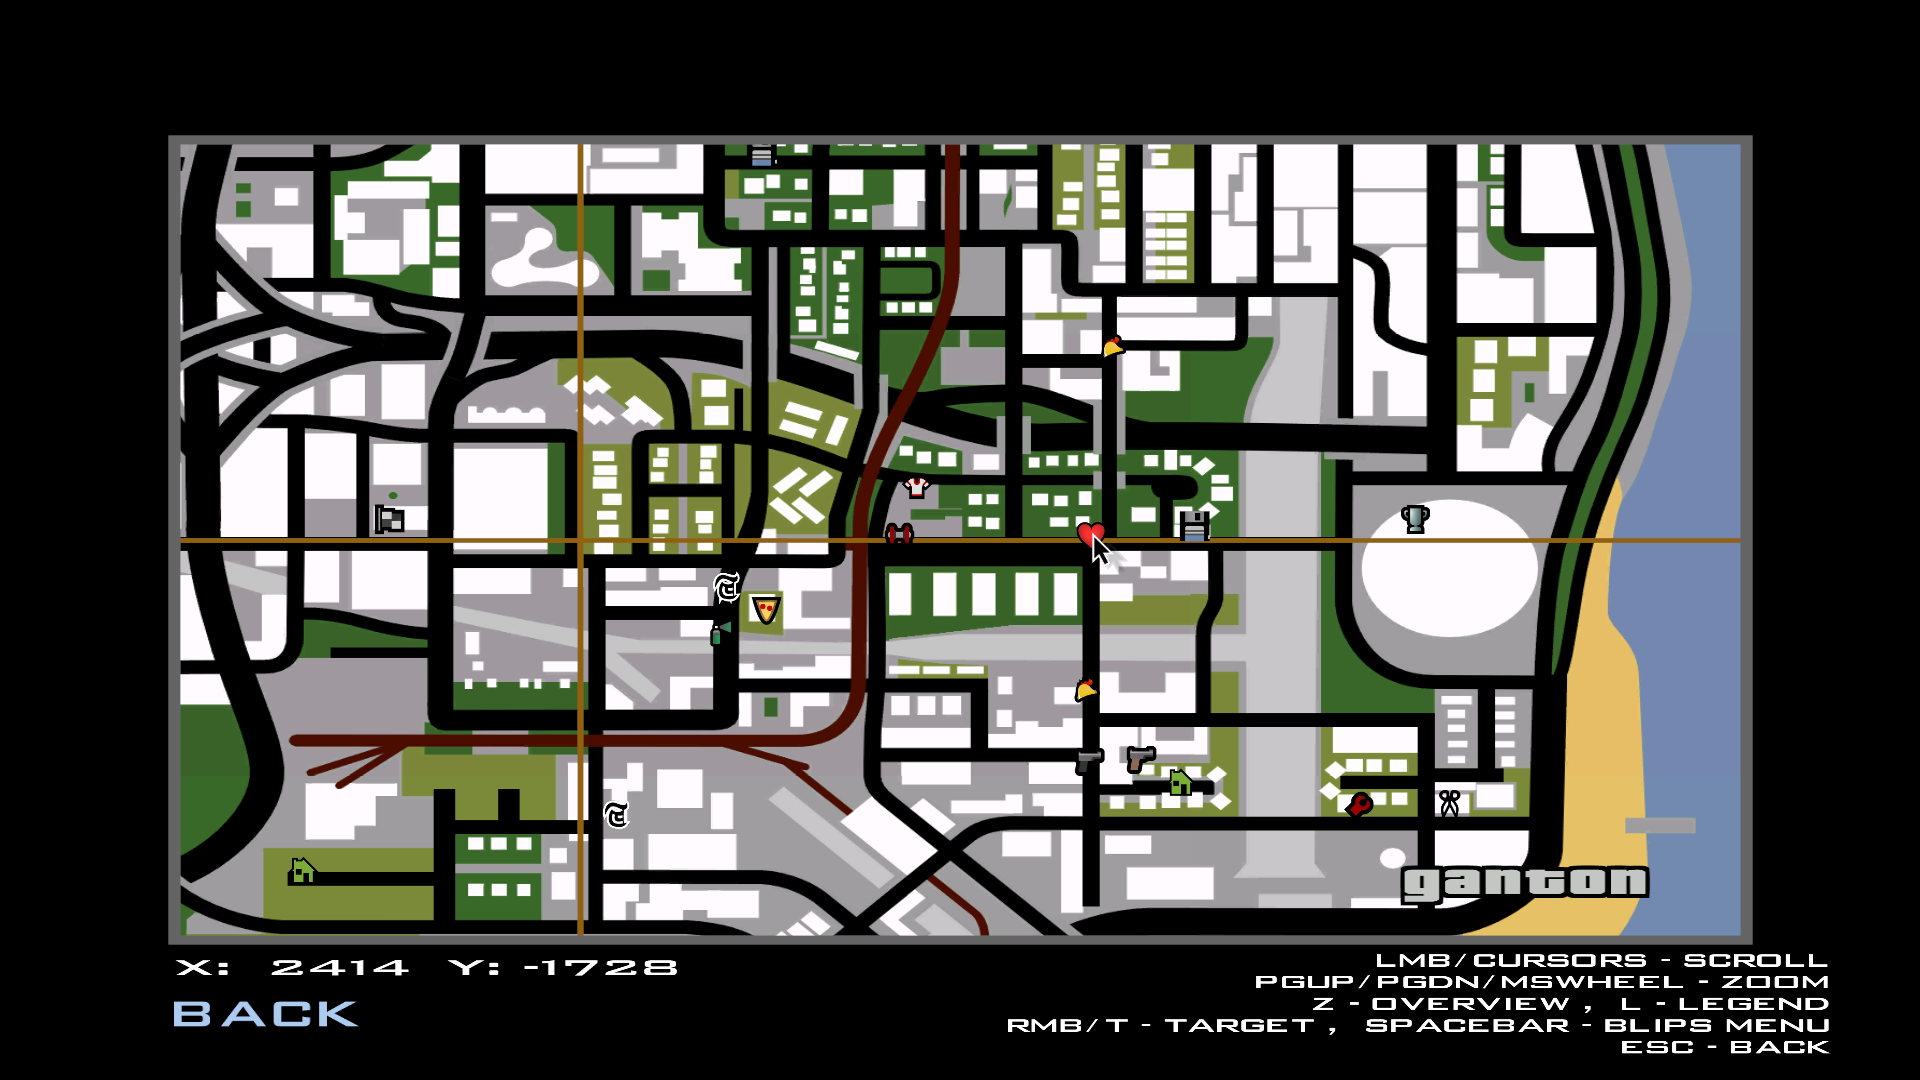
\includegraphics[width= 1\textwidth]{./0img/girlfriendMap.png}
			\subcaption{Map Overview}
		\end{minipage}
		\caption{Second Special Location}
	\end{figure}
	
	\subsubsection*{Incidence Distance Computation}
	\addcontentsline{toc}{subsubsection}{Incidence Distance Computation}
	For the calculation of each incident vertices distances, we will use the distance formula.
	\begin{align}
		\lVert v_{i} - v_{j} \rVert &= \sqrt{\left(v_{i}^{(x)} - v_{j}^{(x)}\right)^{2} + \left(v_{i}^{(y)} - v_{j}^{(y)}\right)^{2} + \left(v_{i}^{(z)} - v_{j}^{(z}\right)^{2}}
		\label{distance_formula}
	\end{align} Where \(v_{i}, v_{j} \in \mathbb{R}^{3} \), which has a 3-dimensional components \((x, y, z)\). To get the value of each components from a certain location [vertex], we shall utilize a modification that will display a real-time coordinate in-game.
	
	\begin{figure}[!h]
		\centering
		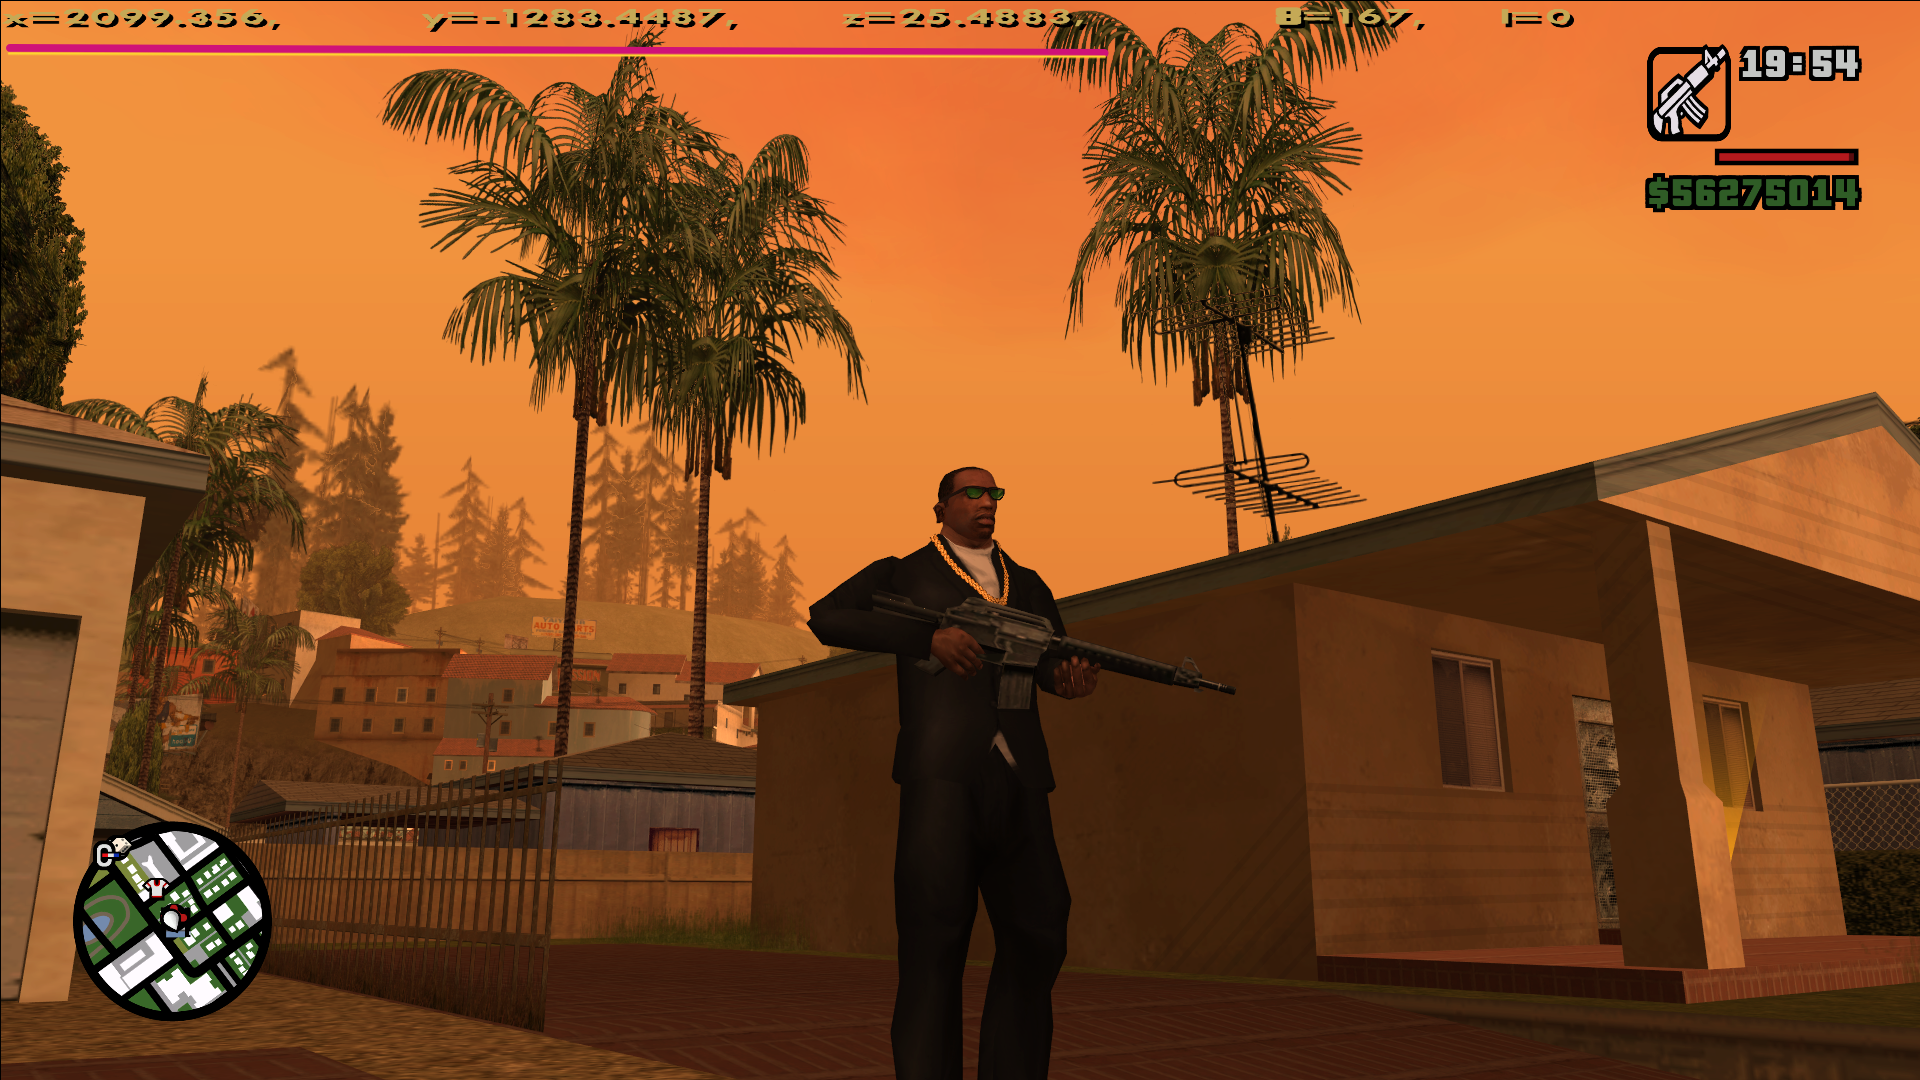
\includegraphics[width=1\textwidth]{./0img/coordinateSystem.png}
		\caption{Coordinate System}
	\end{figure} The top corner highlighted in magenta and yellow represents the current location that our player character resides at. The other two non-important displays \(\theta\) (looks like 8) and \(I\) represents the angle of the player character and if he is inside an interior (house, mall, gym, etc) or in the over-world (outside). 
	
	As to how it is gonna be calculated, the process is straightforward. Go to your desired source location \(v_{i}\), get its coordinates, then go to the sink location \(v_{j}\) and again get its xyz coordinates. Finally use equation (\ref{distance_formula}) to get both of their distance. The weights for all edges can be found at the graph section.
	
	\ifx\graphTheoryPreambleLoaded
\end{document}
\fi